% vim: set tw=78 sts=2 sw=2 ts=8 aw et ai:

One attempt to use steganography for hiding messages in TCP/IP headers was presented in 2010 at ICACTE by a group of Indian researchers.  They had 2 scenarios in mind:

1. Using the Flags section of the IP header, particularly the DF flag, to send 1 or 0 to the receiver, thus prompting an action. This scenario only works if the MF flag is set on 0, which makes the network receivers along the way to ignore the DF flag.  Although this method works, it's not suitable for longer messages because of the number of packets you would have to send over the network.

2. Using the IP identification field to send a message encrypted using chaotic mixing. This method doesn't work if along the way a checker wants the field to contain certain information and it also splits messages into pieces, even smaller ones like "ABC", which can cause suspicion. 

\begin{figure}
  \centering
  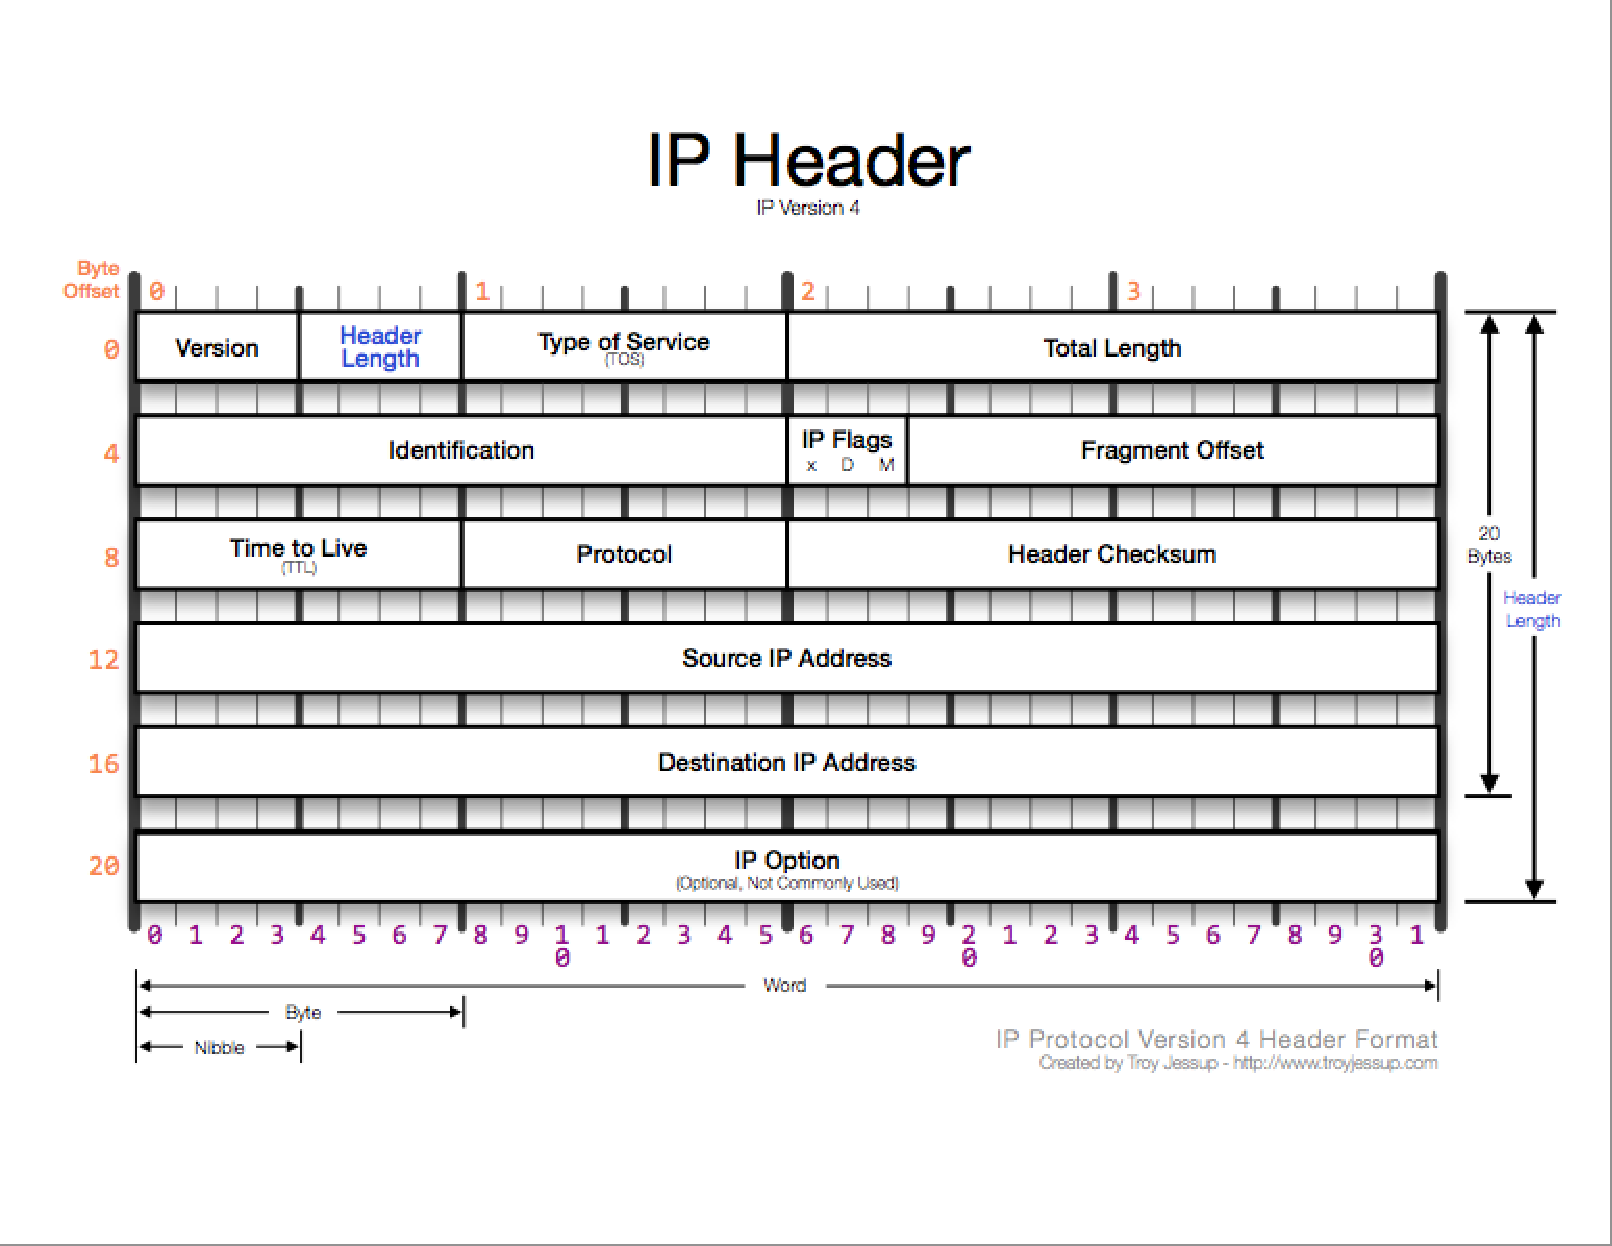
\includegraphics[width=0.5\textwidth]{img/IPHeader}
  \caption{IP header structure}
  \label{fig:related}
\end{figure}
